\PassOptionsToPackage{unicode=true}{hyperref} % options for packages loaded elsewhere
\PassOptionsToPackage{hyphens}{url}
%
\documentclass[ignorenonframetext,]{beamer}
\usepackage{pgfpages}
\setbeamertemplate{caption}[numbered]
\setbeamertemplate{caption label separator}{: }
\setbeamercolor{caption name}{fg=normal text.fg}
\beamertemplatenavigationsymbolsempty
\usepackage{lmodern}
\usepackage{amssymb,amsmath}
\usepackage{ifxetex,ifluatex}
\usepackage{fixltx2e} % provides \textsubscript
\ifnum 0\ifxetex 1\fi\ifluatex 1\fi=0 % if pdftex
  \usepackage[T1]{fontenc}
  \usepackage[utf8]{inputenc}
  \usepackage{textcomp} % provides euro and other symbols
\else % if luatex or xelatex
  \usepackage{unicode-math}
  \defaultfontfeatures{Ligatures=TeX,Scale=MatchLowercase}
\fi
\usetheme[]{CambridgeUS}
\usecolortheme{beaver}
\usefonttheme{structurebold}
% use upquote if available, for straight quotes in verbatim environments
\IfFileExists{upquote.sty}{\usepackage{upquote}}{}
% use microtype if available
\IfFileExists{microtype.sty}{%
\usepackage[]{microtype}
\UseMicrotypeSet[protrusion]{basicmath} % disable protrusion for tt fonts
}{}
\IfFileExists{parskip.sty}{%
\usepackage{parskip}
}{% else
\setlength{\parindent}{0pt}
\setlength{\parskip}{6pt plus 2pt minus 1pt}
}
\usepackage{hyperref}
\hypersetup{
            pdftitle={Choroplethen - Das Paket maptools},
            pdfauthor={Jan-Philipp Kolb},
            pdfborder={0 0 0},
            breaklinks=true}
\urlstyle{same}  % don't use monospace font for urls
\newif\ifbibliography
\usepackage{color}
\usepackage{fancyvrb}
\newcommand{\VerbBar}{|}
\newcommand{\VERB}{\Verb[commandchars=\\\{\}]}
\DefineVerbatimEnvironment{Highlighting}{Verbatim}{commandchars=\\\{\}}
% Add ',fontsize=\small' for more characters per line
\usepackage{framed}
\definecolor{shadecolor}{RGB}{248,248,248}
\newenvironment{Shaded}{\begin{snugshade}}{\end{snugshade}}
\newcommand{\AlertTok}[1]{\textcolor[rgb]{0.94,0.16,0.16}{#1}}
\newcommand{\AnnotationTok}[1]{\textcolor[rgb]{0.56,0.35,0.01}{\textbf{\textit{#1}}}}
\newcommand{\AttributeTok}[1]{\textcolor[rgb]{0.77,0.63,0.00}{#1}}
\newcommand{\BaseNTok}[1]{\textcolor[rgb]{0.00,0.00,0.81}{#1}}
\newcommand{\BuiltInTok}[1]{#1}
\newcommand{\CharTok}[1]{\textcolor[rgb]{0.31,0.60,0.02}{#1}}
\newcommand{\CommentTok}[1]{\textcolor[rgb]{0.56,0.35,0.01}{\textit{#1}}}
\newcommand{\CommentVarTok}[1]{\textcolor[rgb]{0.56,0.35,0.01}{\textbf{\textit{#1}}}}
\newcommand{\ConstantTok}[1]{\textcolor[rgb]{0.00,0.00,0.00}{#1}}
\newcommand{\ControlFlowTok}[1]{\textcolor[rgb]{0.13,0.29,0.53}{\textbf{#1}}}
\newcommand{\DataTypeTok}[1]{\textcolor[rgb]{0.13,0.29,0.53}{#1}}
\newcommand{\DecValTok}[1]{\textcolor[rgb]{0.00,0.00,0.81}{#1}}
\newcommand{\DocumentationTok}[1]{\textcolor[rgb]{0.56,0.35,0.01}{\textbf{\textit{#1}}}}
\newcommand{\ErrorTok}[1]{\textcolor[rgb]{0.64,0.00,0.00}{\textbf{#1}}}
\newcommand{\ExtensionTok}[1]{#1}
\newcommand{\FloatTok}[1]{\textcolor[rgb]{0.00,0.00,0.81}{#1}}
\newcommand{\FunctionTok}[1]{\textcolor[rgb]{0.00,0.00,0.00}{#1}}
\newcommand{\ImportTok}[1]{#1}
\newcommand{\InformationTok}[1]{\textcolor[rgb]{0.56,0.35,0.01}{\textbf{\textit{#1}}}}
\newcommand{\KeywordTok}[1]{\textcolor[rgb]{0.13,0.29,0.53}{\textbf{#1}}}
\newcommand{\NormalTok}[1]{#1}
\newcommand{\OperatorTok}[1]{\textcolor[rgb]{0.81,0.36,0.00}{\textbf{#1}}}
\newcommand{\OtherTok}[1]{\textcolor[rgb]{0.56,0.35,0.01}{#1}}
\newcommand{\PreprocessorTok}[1]{\textcolor[rgb]{0.56,0.35,0.01}{\textit{#1}}}
\newcommand{\RegionMarkerTok}[1]{#1}
\newcommand{\SpecialCharTok}[1]{\textcolor[rgb]{0.00,0.00,0.00}{#1}}
\newcommand{\SpecialStringTok}[1]{\textcolor[rgb]{0.31,0.60,0.02}{#1}}
\newcommand{\StringTok}[1]{\textcolor[rgb]{0.31,0.60,0.02}{#1}}
\newcommand{\VariableTok}[1]{\textcolor[rgb]{0.00,0.00,0.00}{#1}}
\newcommand{\VerbatimStringTok}[1]{\textcolor[rgb]{0.31,0.60,0.02}{#1}}
\newcommand{\WarningTok}[1]{\textcolor[rgb]{0.56,0.35,0.01}{\textbf{\textit{#1}}}}
\usepackage{longtable,booktabs}
\usepackage{caption}
% These lines are needed to make table captions work with longtable:
\makeatletter
\def\fnum@table{\tablename~\thetable}
\makeatother
\usepackage{graphicx,grffile}
\makeatletter
\def\maxwidth{\ifdim\Gin@nat@width>\linewidth\linewidth\else\Gin@nat@width\fi}
\def\maxheight{\ifdim\Gin@nat@height>\textheight\textheight\else\Gin@nat@height\fi}
\makeatother
% Scale images if necessary, so that they will not overflow the page
% margins by default, and it is still possible to overwrite the defaults
% using explicit options in \includegraphics[width, height, ...]{}
\setkeys{Gin}{width=\maxwidth,height=\maxheight,keepaspectratio}
% Prevent slide breaks in the middle of a paragraph:
\widowpenalties 1 10000
\raggedbottom
\setbeamertemplate{part page}{
\centering
\begin{beamercolorbox}[sep=16pt,center]{part title}
  \usebeamerfont{part title}\insertpart\par
\end{beamercolorbox}
}
\setbeamertemplate{section page}{
\centering
\begin{beamercolorbox}[sep=12pt,center]{part title}
  \usebeamerfont{section title}\insertsection\par
\end{beamercolorbox}
}
\setbeamertemplate{subsection page}{
\centering
\begin{beamercolorbox}[sep=8pt,center]{part title}
  \usebeamerfont{subsection title}\insertsubsection\par
\end{beamercolorbox}
}
\AtBeginPart{
  \frame{\partpage}
}
\AtBeginSection{
  \ifbibliography
  \else
    \frame{\sectionpage}
  \fi
}
\AtBeginSubsection{
  \frame{\subsectionpage}
}
\setlength{\emergencystretch}{3em}  % prevent overfull lines
\providecommand{\tightlist}{%
  \setlength{\itemsep}{0pt}\setlength{\parskip}{0pt}}
\setcounter{secnumdepth}{0}

% set default figure placement to htbp
\makeatletter
\def\fps@figure{htbp}
\makeatother


\title{Choroplethen - Das Paket maptools}
\author{Jan-Philipp Kolb}
\date{22 Oktober 2018}

\begin{document}
\frame{\titlepage}

\begin{frame}[fragile]{Das Paket \texttt{maptools}}
\protect\hypertarget{das-paket-maptools}{}

\begin{itemize}
\tightlist
\item
  Datensatz wrld\_simpl aus dem Paket \texttt{maptools}
\item
  Polygone für fast alle Staaten der Erde
\end{itemize}

\begin{Shaded}
\begin{Highlighting}[]
\KeywordTok{library}\NormalTok{(maptools)}
\KeywordTok{data}\NormalTok{(wrld_simpl)}
\end{Highlighting}
\end{Shaded}

\begin{longtable}[]{@{}lllrr@{}}
\toprule
& ISO2 & NAME & AREA & POP2005\tabularnewline
\midrule
\endhead
ATG & AG & Antigua and Barbuda & 44 & 83039\tabularnewline
DZA & DZ & Algeria & 238174 & 32854159\tabularnewline
AZE & AZ & Azerbaijan & 8260 & 8352021\tabularnewline
ALB & AL & Albania & 2740 & 3153731\tabularnewline
ARM & AM & Armenia & 2820 & 3017661\tabularnewline
AGO & AO & Angola & 124670 & 16095214\tabularnewline
\bottomrule
\end{longtable}

\end{frame}

\begin{frame}[fragile]{Hallo Welt}
\protect\hypertarget{hallo-welt}{}

\begin{Shaded}
\begin{Highlighting}[]
\KeywordTok{plot}\NormalTok{(wrld_simpl)}
\end{Highlighting}
\end{Shaded}

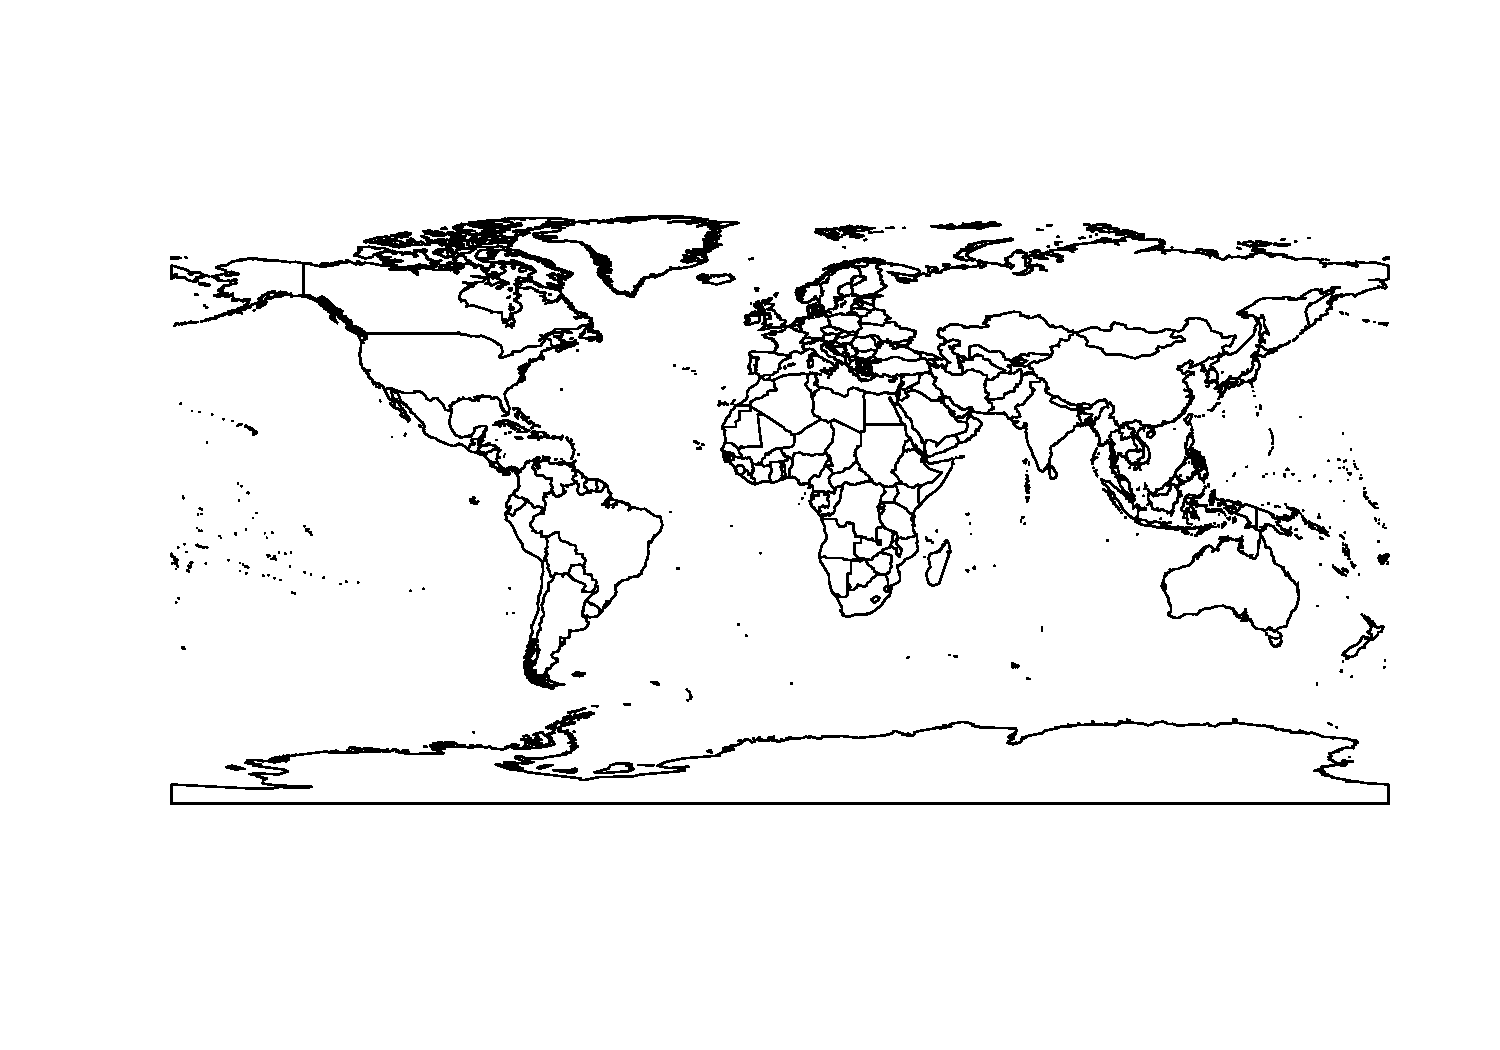
\includegraphics{Choroplethen_files/figure-beamer/unnamed-chunk-3-1.pdf}

\end{frame}

\begin{frame}[fragile]{\href{https://datahub.io/core/gini-index\#data}{Daten
zum Gini Index}}
\protect\hypertarget{daten-zum-gini-index}{}

\begin{Shaded}
\begin{Highlighting}[]
\NormalTok{gini <-}\StringTok{ }\KeywordTok{read.csv}\NormalTok{(}\StringTok{"../data/gini-index_csv.csv"}\NormalTok{)}
\end{Highlighting}
\end{Shaded}

\begin{longtable}[]{@{}llrr@{}}
\toprule
Country.Name & Country.Code & Year & Value\tabularnewline
\midrule
\endhead
Albania & ALB & 1996 & 27.0\tabularnewline
Albania & ALB & 2002 & 31.7\tabularnewline
Albania & ALB & 2005 & 30.6\tabularnewline
Albania & ALB & 2008 & 30.0\tabularnewline
Albania & ALB & 2012 & 29.0\tabularnewline
Algeria & DZA & 1988 & 40.2\tabularnewline
\bottomrule
\end{longtable}

\end{frame}

\begin{frame}[fragile]{Der Gini Index im Jahr 2012}
\protect\hypertarget{der-gini-index-im-jahr-2012}{}

\begin{Shaded}
\begin{Highlighting}[]
\NormalTok{gini12 <-}\StringTok{ }\NormalTok{gini[gini}\OperatorTok{$}\NormalTok{Year}\OperatorTok{==}\DecValTok{2012}\NormalTok{,]}
\KeywordTok{summary}\NormalTok{(gini12}\OperatorTok{$}\NormalTok{Value)}
\end{Highlighting}
\end{Shaded}

\begin{verbatim}
##    Min. 1st Qu.  Median    Mean 3rd Qu.    Max. 
##   24.70   29.80   35.10   36.15   41.40   57.40
\end{verbatim}

\end{frame}

\begin{frame}[fragile]{Die Daten matchen}
\protect\hypertarget{die-daten-matchen}{}

\begin{Shaded}
\begin{Highlighting}[]
\NormalTok{ind <-}\StringTok{ }\KeywordTok{match}\NormalTok{(gini12}\OperatorTok{$}\NormalTok{Country.Code,wrld_simpl}\OperatorTok{$}\NormalTok{ISO3)}
\NormalTok{ind2 <-}\StringTok{ }\NormalTok{ind[}\OperatorTok{!}\KeywordTok{is.na}\NormalTok{(ind)]}
\end{Highlighting}
\end{Shaded}

\begin{Shaded}
\begin{Highlighting}[]
\NormalTok{ginimap <-}\StringTok{ }\NormalTok{wrld_simpl[ind2,]}
\NormalTok{ginimap}\OperatorTok{@}\NormalTok{data}\OperatorTok{$}\NormalTok{gini12 <-}\StringTok{ }\NormalTok{gini12}\OperatorTok{$}\NormalTok{Value[}\OperatorTok{!}\KeywordTok{is.na}\NormalTok{(ind)]}
\end{Highlighting}
\end{Shaded}

\end{frame}

\begin{frame}[fragile]{Die Daten plotten}
\protect\hypertarget{die-daten-plotten}{}

\begin{Shaded}
\begin{Highlighting}[]
\KeywordTok{library}\NormalTok{(sp)}
\KeywordTok{spplot}\NormalTok{(ginimap,}\StringTok{"gini12"}\NormalTok{)}
\end{Highlighting}
\end{Shaded}

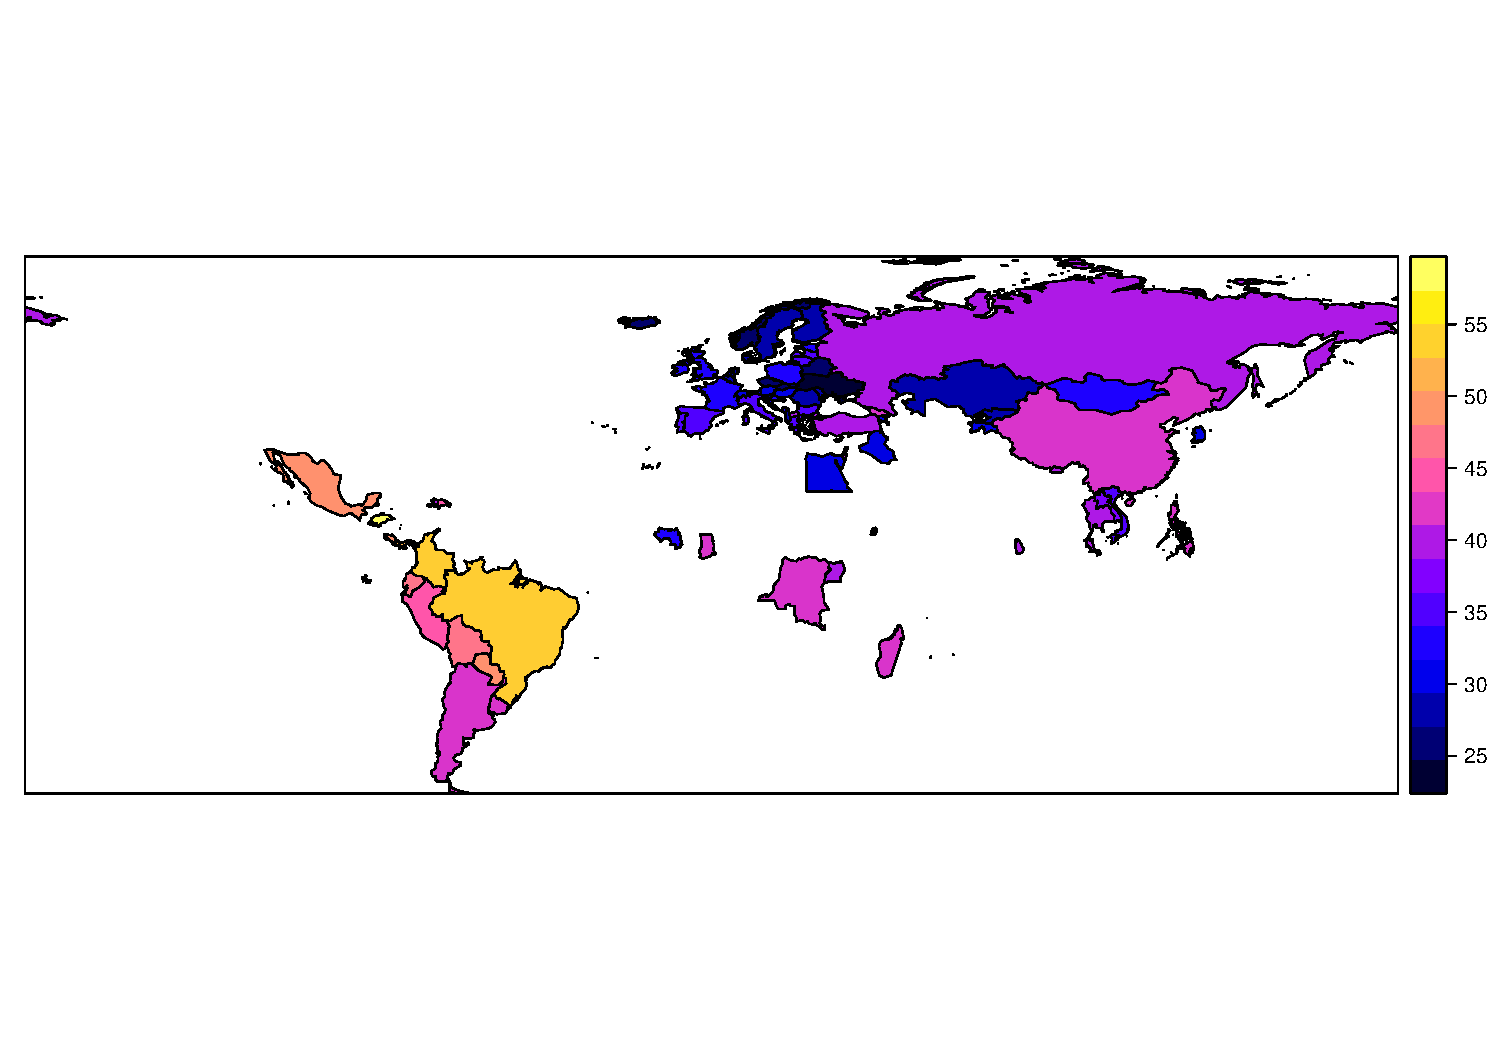
\includegraphics{Choroplethen_files/figure-beamer/unnamed-chunk-9-1.pdf}

\end{frame}

\begin{frame}{Aufgabe}
\protect\hypertarget{aufgabe}{}

\begin{itemize}
\tightlist
\item
  Lade Datensatz xy herunter
\item
  Erzeuge mit der Variable yx folgende Karte:
\end{itemize}

\end{frame}

\end{document}
